\documentclass[preview]{standalone}

\usepackage{amsmath}
\usepackage{amssymb}
\usepackage{stellar}
\usepackage{definitions}
\usepackage{bettelini}
\usepackage{tikz}

\begin{document}

\id{curves-basic-results-definitions}
\genpage

\section{Basic results}

\begin{snippetproposition}{curve-equivalence-same-support}{}
    Let \(\varphi_1 \colon I_1 \fromto \realnumbers^n\)
    and \(\varphi_2 \colon I_2 \fromto \realnumbers^n\) be two \curve[curves].
    If \(\varphi_1 \curveequivalent \varphi_2\) then
    \(\varphi_1\) and \(\varphi_2\) have the same \curve[support].
\end{snippetproposition}

\begin{snippetproposition}{lipschitz-curve-is-rectifiable}{}
    Let \(\varphi \colon I \fromto \realnumbers^n\) be a \curve that is lipschitz.
    Then, \(\varphi\) is rectifiable.
\end{snippetproposition}

\begin{snippetproof}{lipschitz-curve-is-rectifiable-proof}{lipschitz-curve-is-rectifiable}{}
    We have that
    \[
        \forall t,s \in I, ||\varphi(s)-\varphi(t)|| \leq L|t-s|
    \]
    thus
    \begin{align*}
        \curvelength(\varphi, P) &= \sum_{i=1}^n ||\varphi(t_i) - \varphi(t_{i-2})|| \\
        &\leq \sum_{i=1}^n L|t_i-t_{i-1}| = \curvelength(b-a)
    \end{align*}
    meaning that \(\curvelength(\varphi) \leq \curvelength(b-a)\).
\end{snippetproof}

\begin{snippetexample}{curve-length-example1}{}
    Let \(\varphi(t) = (\cos t, \sin t)\) defined on \(I = [0, \pi]\).
    We have
    \begin{align*}
        ||\varphi(t)-\varphi(s)|| &= {\left\{
            {\left(\cos t - \cos s\right)}^2
            +
            {\left(\sin t - \sin s\right)}^2
        \right\}}^{1/2} \\
        &= {\left\{
            {(-\sin \alpha(t-s))}^2
            + 
            {(\cos \beta(t-s))}^2
        \right\}}^{1/2} \\
        & \leq \sqrt{2} |t-s|
    \end{align*}
    We thus have that \(\curvelength(\varphi) \leq \sqrt{2}\pi\).
\end{snippetexample}

\begin{snippetproposition}{curve-length-upper-bound}{}
    \begin{align*}
        \left|\left|
            \integral[a][b][\varphi(t)][t]
        \right|\right|
        \leq \integral[a][b][||\varphi(t)||][t]
    \end{align*}
    where the integral of a vector is the vector of the integrals.
\end{snippetproposition}

\begin{snippetproof}{curve-length-upper-bound-proof}{curve-length-upper-bound}{}
    Let \[
        v = \left(\integral[a][b][\varphi_1(t)][t], \cdots, \integral[a][b][\varphi_n(t)][t]\right)
    \]
    then
    \begin{align*}
        \left|\left|
            \integral[a][b][\varphi(t)][t]
        \right|\right| &= ||v||^2 = \langle v,v \rangle
        = \sum_{i=1}^n v_i \integral[a][b][\varphi_i(t)][t] \\
        &= \integral[a][b][\sum_{i=1}^n v_i\varphi_i(t)][t] \\
        &= \integral[a][b][\langle v, \varphi(t)\rangle ][t] \\
        &\leq \integral[a][b][||v|| \cdot ||\varphi(t)||][t] \\
        &= ||v|| \integral[a][b][||\varphi(t)||][t]
    \end{align*}
\end{snippetproof}

\section{Curve length formula}

\begin{snippettheorem}{curve-length-formula-theorem}{Curve length formula}
    Let \(\varphi \colon I \to \realnumbers^n\) with \(\varphi \in \continuityclass^1(I)\).
    Then, \(\varphi\) is rectifiable and
    \[
        \curvelength(\varphi) = \integral[a][b][||\varphi'(t)||][t]
    \]
\end{snippettheorem}

\begin{snippetproof}{curve-length-formula-proof}{curve-length-formula}{Curve length formula}
    Clearly the \function is lipschitz.
    \begin{enumerate}
        \item \begin{align*}
            \curvelength(\varphi, P) &= \sum_{i=1}^n ||\varphi(t_i) - \varphi(t_{i-1})|| \\
            &= \sum_{i=1}^n \left|\left|
                \integral[t_{i-1}][t_i][\varphi'(t)][t]
            \right|\right| \\
            &\leq \sum_{i=1}^n \integral[t_{i-1}][t_i][||\varphi'(t)||][t] \\
            &= \integral[a][b][||\varphi'(t)||][t]
        \end{align*}
        We thus have
        \begin{align*}
            \curvelength(\varphi) \leq \integral[a][b][||\varphi'(t)||][t]
        \end{align*}
        \item we will now prove the other direction. Since \([a,b]\) is compact and \(\varphi\)
        is continuous, then it is uniformly continuous. Hence,
        \[
            \forall \varepsilon > 0, \exists \delta>0 \,|\,
            \delta > |t-s| \implies ||\varphi(t) - \varphi(s)|| < \varepsilon
        \]
        We now take a \partition \(P\) such that \(|t_i - t_{i-1} < \delta\). We then have
        \begin{align*}
            \integral[t_{i-1}][t_i][||\varphi'(t)||][t]
            &= \integral[t_{i-1}][t_i][||\varphi'(t) - \varphi'(t_{i-1}) + \varphi'(t_{i-1})||][t] \\
            &\leq \integral[t_{i-1}][t_i][||\varphi'(t) - \varphi'(t_{i-1})||][t]
            + \integral[t_{i-1}][t_i][||\varphi'(t_{i-1})||][t] \\
            &\leq \varepsilon(t_i - t_{i-1}) + \varphi'(t_{i-1})(t_i - t_{i-1})
            = \varepsilon(t_i - t_{i-1}) + ||(t_i - t_{i-1})\varphi'(t_{i-1})|| \\
            &= \varepsilon(t_i - t_{i-1}) + \left|\left|\,
                \integral[t_{i-1}][t_i][\varphi'(t_{i-1})][t]
            \right|\right| =
            \varepsilon(t_i - t_{i-1}) + \left|\left|\,
            \integral[t_{i-1}][t_i][\varphi'(t_{i-1}) - \varphi'(t) - \varphi'(t)][t]
        \right|\right| \\
        &= \varepsilon(t_i - t_{i-1}) + \left|\left|\,
            \integral[t_{i-1}][t_i][\varphi'(t_{i-1}) - \varphi'(t)][t]
            \integral[t_{i-1}][t_i][\varphi'(t)][t]
        \right|\right| \\
        &\leq \varepsilon(t_i - t_{i-1}) + \left|\left|\,
            \integral[t_{i-1}][t_i][\varphi'(t_{i-1}) - \varphi'(t)][t]
        \right|\right| +
        \left|\left|\,
            \integral[t_{i-1}][t_i][\varphi'(t)][t]
        \right|\right| \\
        &\leq \varepsilon(t_i - t_{i-1}) \integral[t_{i-1}][t_i][\varphi'(t_{i-1}) - \varphi'(t)][t]
        + ||\varphi(t_i) - \varphi(t_{i-1})|| \\
        &\leq 2\varepsilon(t_i - t_{i-1}) + ||\varphi(t_i) - \varphi(t_{i-1})||
        \end{align*}
        by adding we obtain
        \begin{align*}
            \integral[a][b][||\varphi'(t)||][t] &= \sum_{i=1}^n \integral[t_{i-1}][t_i][||\varphi'(t)||][t] \\
            &\leq 2\varepsilon(b-a) + \sum_{i=1}^n ||\varphi(t_i) - \varphi(t_{i-1})|| \\
            &\leq 2\varepsilon + \curvelength(\varphi) \\
            \integral[a][b][||\varphi'(t)||][t] &\leq \curvelength(\varphi)
        \end{align*}
    \end{enumerate}
    meaning that the equivalence is true.
\end{snippetproof}

\begin{snippet}{curve-length-formula-bidimensional-case}
    For the bidimensional case \(\varphi(t) = (t, f(t))\) we have
    \[
        \integral[a][b][||\varphi'(t)||][t] = \integral[a][b][||(1, f'(t))||][t]
        = \integral[a][b][\sqrt{1 + {\frac{df}{dt}}^2}][t]
    \]
\end{snippet}

\begin{snippetexample}{non-rectifiable-curve-example1}{}
    The \curve \(\varphi\colon [0,1] \to \realnumbers^2\)
    defined as a segment which bounces between the two bisector at the point \(1/i\),
    and coming closer to the origin, is not rectifiable.
    \begin{center}
        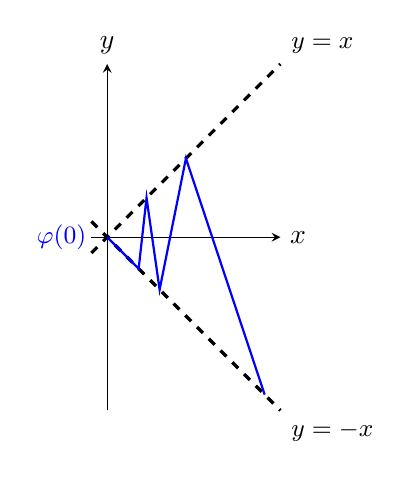
\begin{tikzpicture}[scale=2,>=stealth]
          \draw[->] (-0.1,0) -- (1.1,0) node[right] {$x$};
          \draw[->] (0,-1.1) -- (0,1.1) node[above] {$y$};
      
          \draw[dashed,very thick,black] (-0.1,-0.1) -- (1.1,1.1) node[above right] {\small $y=x$};
          \draw[dashed,very thick,black] (-0.1,0.1) -- (1.1,-1.1) node[below right] {\small $y=-x$};
      
          \draw[thick, blue]
            (1.000,-1.000) --
            (0.500, 0.500) --
            (0.333,-0.333) --
            (0.250, 0.250) --
            (0.200,-0.200) --
            (0,0);
      
          \node[blue,left=4pt] at (0,0) {\small $\varphi(0)$};
        \end{tikzpicture}
    \end{center}
    Consider the \partition \(P = \{0, \frac{1}{n}, \frac{1}{n-1}, \cdots, \frac{1}{2}, 1\}\)
    which are \(n+1\) point.
    Consider \todo
    %\begin{align*}
    %    ||\varphi(t_i) - \varphi(t_{i-1})||
    %    &= \left|\left|\varphi\left(\frac{1}{i}\right)-\varphi\left(\frac{1}{i-1}\right)\right|\right| \\
    %    &= \left|\left|\left(\frac{1}{i}, \frac{{(-1)}^{-1}}{i}\right)
    %    - \left(\frac{1}{i-1}, \frac{{(-1)}^{i-1}}{i-1}\right)\right|\right| \\
    %    &= {\left\{
    %        {\left(\frac{1}{i} - \frac{1}{i-1}\right)}^2 +
    %        {\left(\frac{{(-1)}^i}{i} - \frac{{(-1)}^{i-1}}{i-1}\right)}^2
    %    \right\}}^{1/2} \\
    %    &\geq {\left({\left(\frac{1}{i} + \frac{1}{i-1}\right)}^2\right)}^{1/2}
    %    = \frac{1}{i} + \frac{1}{i-1} \geq \frac{2}{i}
    %\end{align*}
    then, the sum
    \begin{align*}
        \sum_{i=1}^n ||\varphi(t_i) - \varphi(t_{i-1})||
        &\geq \sum_{i=1}^n \frac{2}{i}
    \end{align*}
    diverges for \(n \to \infty\).
\end{snippetexample}

\end{document}